\section{Introduction}
NEXT-DEMO is a high-pressure xenon TPC contained within a cylindrical stainless-steel pressure vessel of diameter 30~cm and length 60~cm which was designed to operate at 10~bar. The TPC itself is defined by three metallic wire grids --- called \emph{cathode}, \emph{gate} and \emph{anode} --- which define the two active regions: the 30-cm long \emph{drift region}, between cathode and gate with a  drift field of typically 500~V~cm$^{-1}$; and the 5 mm long \emph{EL region}, between gate and anode.  The electric field is created by supplying a large negative voltage to the cathode, then degrading it using a series of metallic rings of 30 cm diameter spaced 5 mm and connected via 0.5~G$\Omega$ resistors (shown in figure~\ref{fig:TPC}).  The gate is at negative voltage so that a moderate electric field of typically 2$\mathrm{kV~cm^{-1}~bar^{-1}}$ --- is created between the gate and the anode, which is at ground. A set of six panels made of PTFE (Teflon) coated with tetraphenyl-butadiene (TPB) are mounted inside the electric-field cage forming a \emph{light tube} of hexagonal cross section with an apothem length of 8~cm. 


%%%%%%%%%%
\begin{figure}
\centering
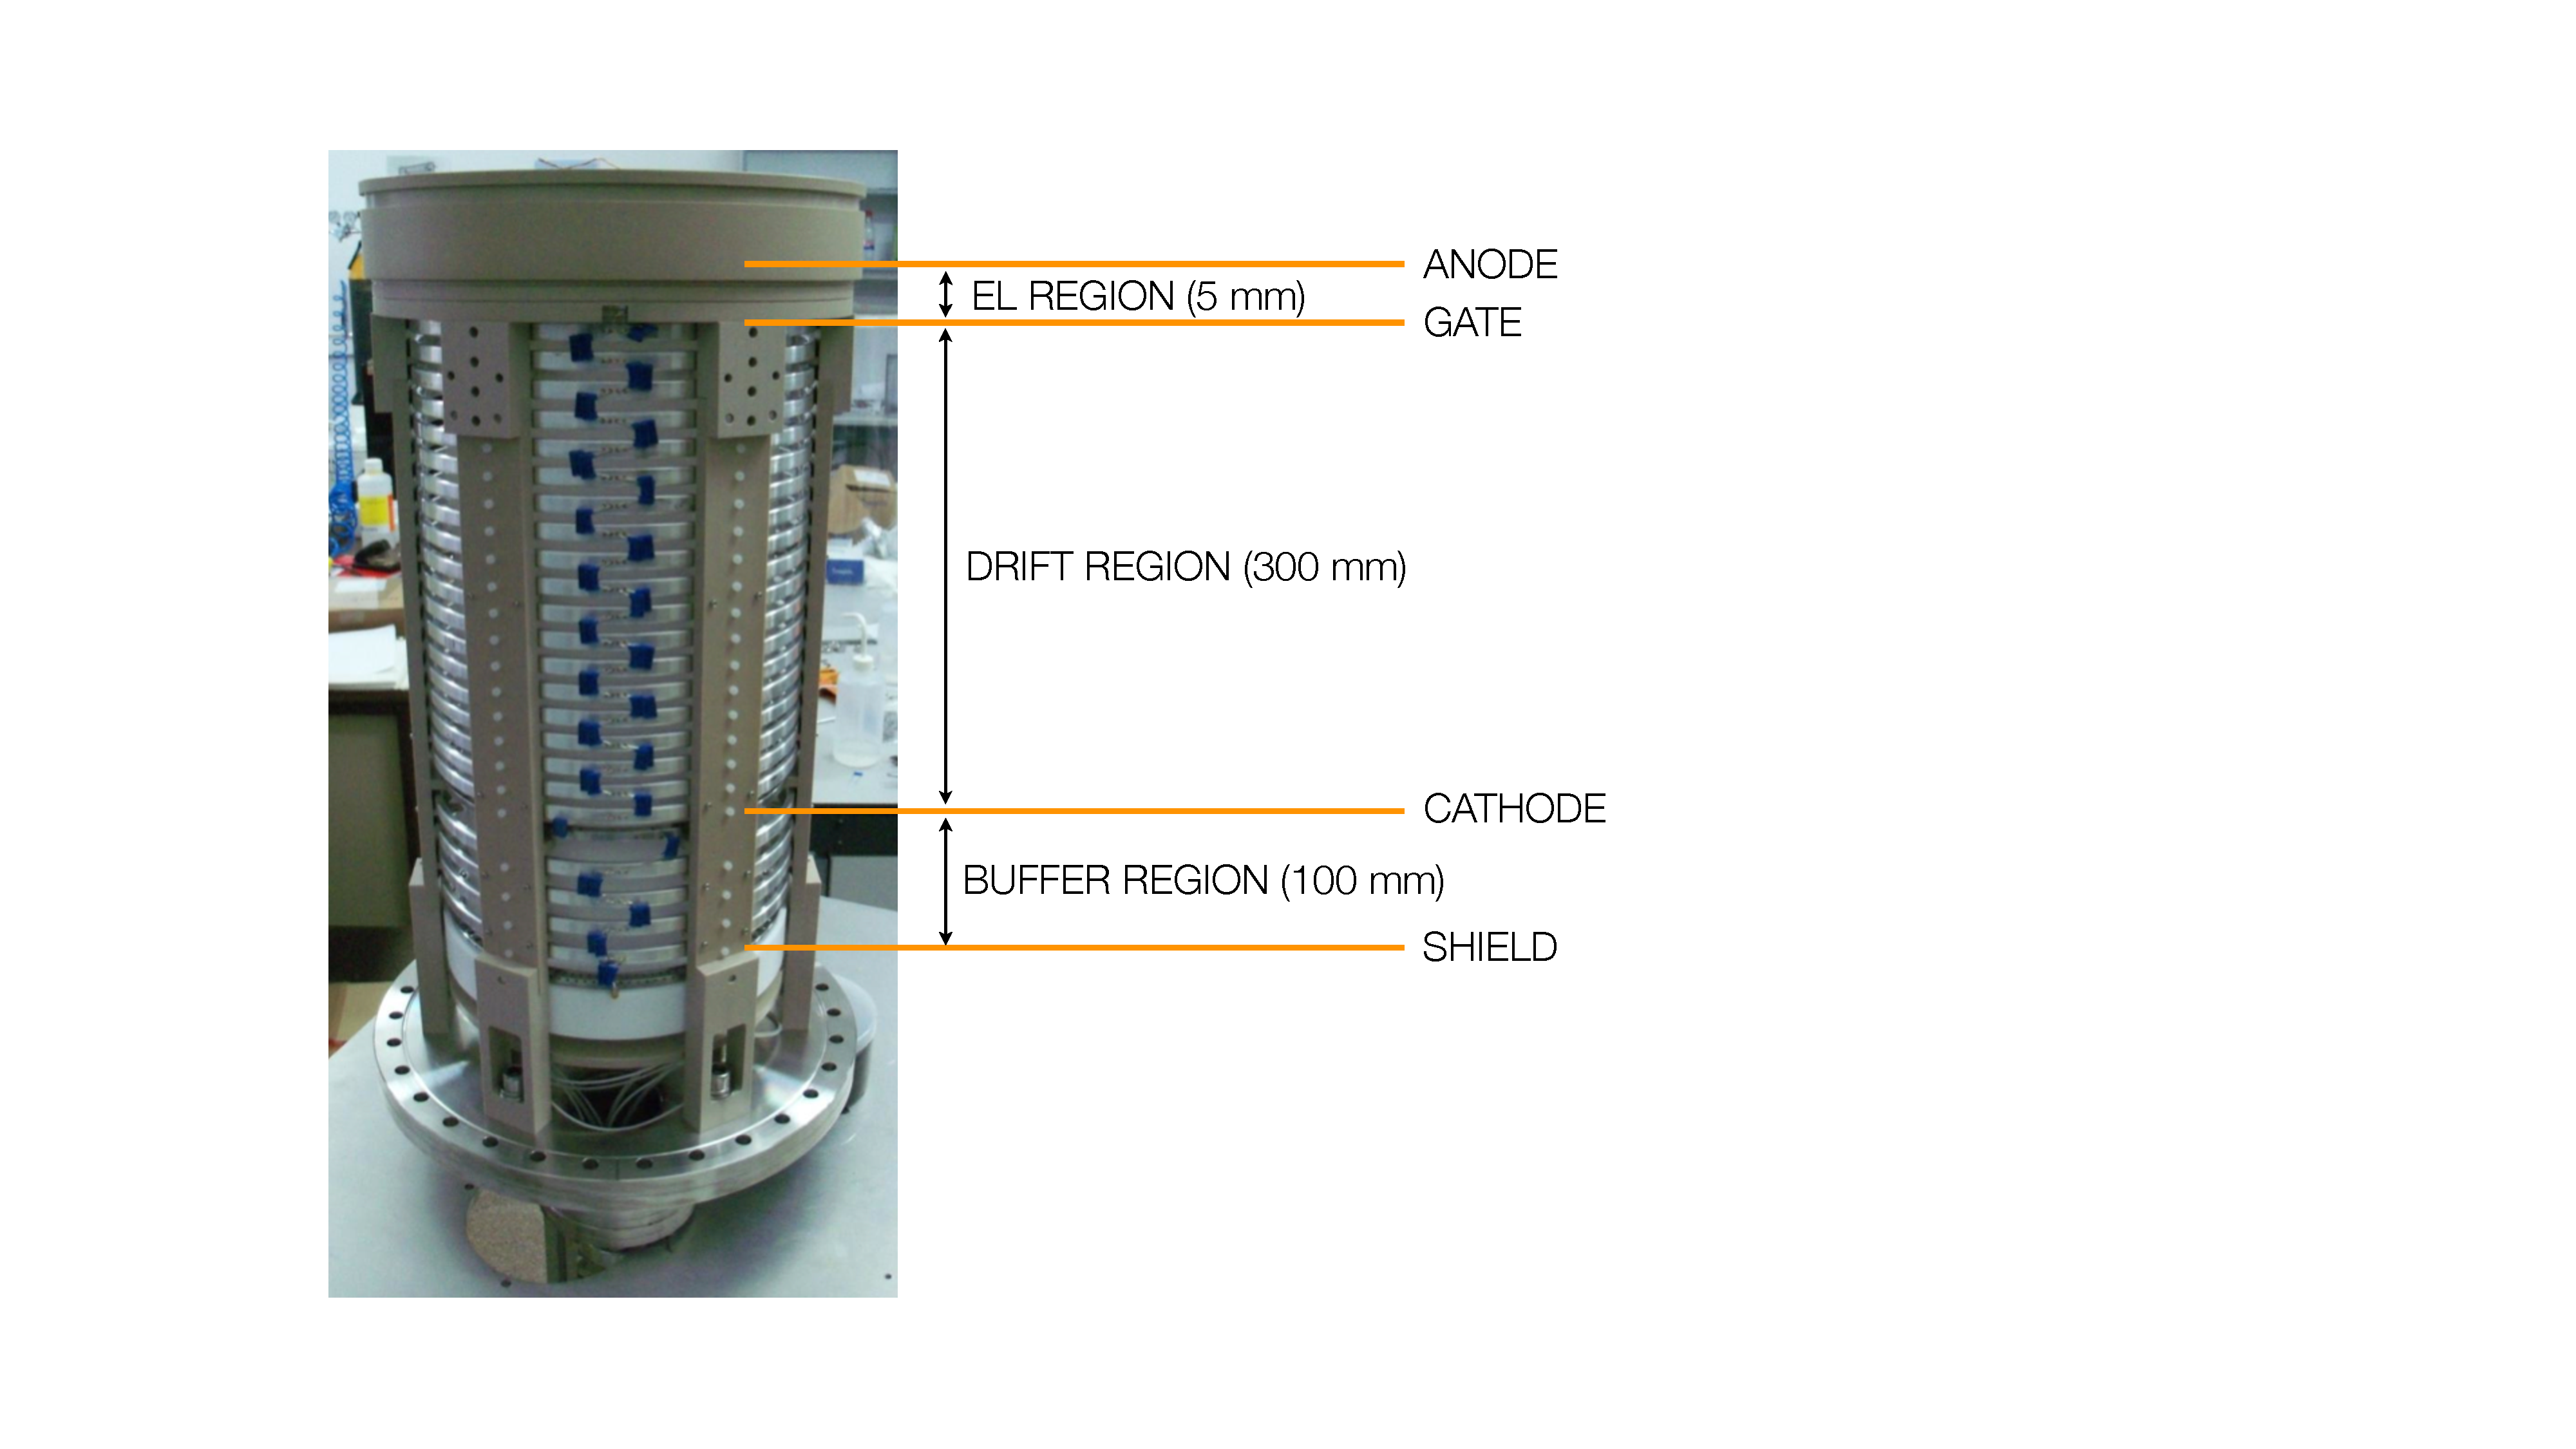
\includegraphics[width=0.75\textwidth]{img/FieldCage.pdf}
\caption{External view of the time projection chamber mounted on one end-cap. The approximate positions of the different regions of the TPC are indicated.} \label{fig:TPC}
\end{figure}
%%%%%%%%%%


The NEXT-DEMO detector has been operating continuously at IFIC (Figure \ref{fig:cleanroom} shows the NEXT-DEMO detector in the experimental are at IFIC ) during the last three years (2011-2014). Its operation and results has been crucial to fully demonstrate the capabilities of the NEXT technology for the search of the neutrinoless double beta decay process. Furthermore, the operation, devoid of any significant incidence has shown the robustness of the system. 

%%%%%%%%%%
\begin{figure}
\centering
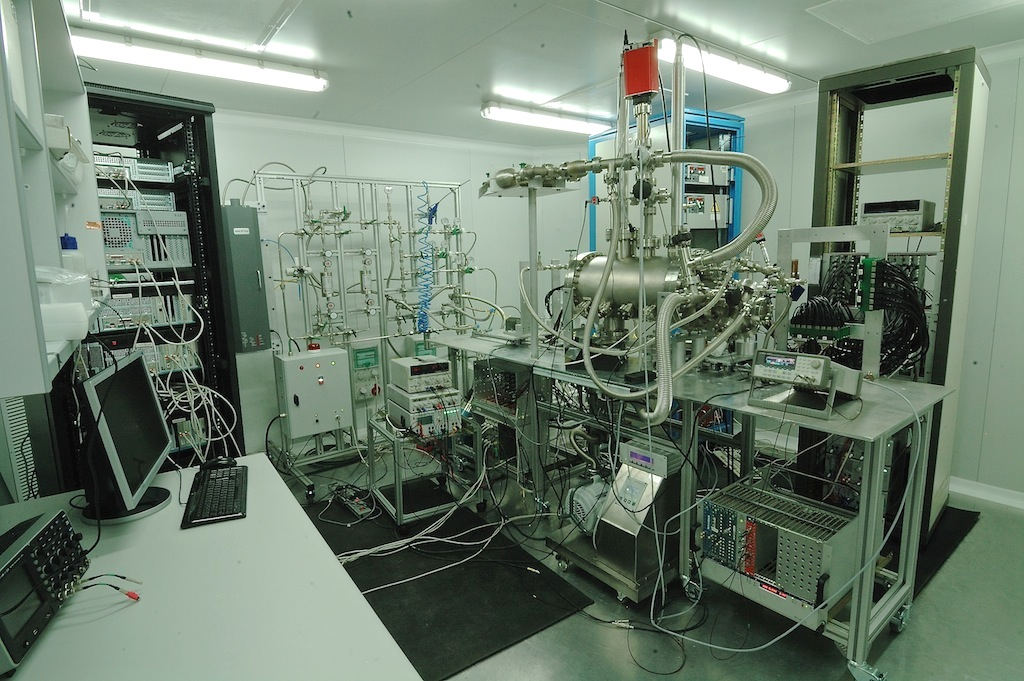
\includegraphics[width=0.75\textwidth]{img/NextDemo_cleanroom.jpg}
\caption{Picture of the NEXT-DEMO detector in the experimental area at IFIC with all the different systems needed for its operation: Gas system, High voltage modules and electronics.} \label{fig:cleanroom}
\end{figure}
%%%%%%%%%%

We propose to use NEXT-DEMO to demonstrate the possibility to operate the NEXT experiment inside a magnetic field of relatively high intensity ($\sim$ 0.5 Tesla). Recent Monte Carlo studies show that the separation between signal and background in the search for neutrinoless double beta decay can be improved by one order of magnitude measuring the sign of the electrons emitted in the decay. However, operation in magnetic field requires a number of upgrades to the current technology (including substituting the PMTs used to measure the event energy by large-area SiPMs and the use of small amounts of CO$_2$ to reduce transverse and longitudinal diffusion) which must be demonstrated experimentally.  

Consequently, we would like to carry out a series of tests at CERN. We propose to place an upgraded version of  NEXT-DEMO detector inside the HARP magnet (TPC90) and operate the detector in various configurations of pressure and magnetic field in order to understand operation in magnetic field and to confirm our Monte Carlo results.
We propose to carry out those tests in 2016, with a possible extension to 2017. 

This document describes at some depth the system that we propose to bring to CERN, including safety aspects. 
